\documentclass{beamer}
\usepackage{ctex, hyperref}
\usepackage[T1]{fontenc}
% 导入额外的 LaTeX 包
\usepackage{latexsym,amsmath,xcolor,multicol,booktabs,calligra}  % 数学符号、公式、颜色、多列、表格等包
\usepackage{graphicx,pstricks,listings,stackengine}  % 图形、PostScript 绘图、代码列表、堆叠等包
\usepackage{subcaption}  % 支持子图功能

% 设置文档信息
\author{董霁兴 \quad 杨成鑫}  % 作者信息
\title{端侧轻量级人脸检测模型对比研究与性能评估}  % 标题
\institute{山东师范大学信息科学与工程学院}  % 机构
\date{2024 年 12 月 17 日}  % 日期
\usepackage{bjtu}  % 使用北京交通大学主题

% 定义一些命令和颜色
\def\cmd#1{\texttt{\color{red}\footnotesize $\backslash$#1}}  % 用于显示命令
\def\env#1{\texttt{\color{blue}\footnotesize #1}}  % 用于显示环境
\definecolor{deepblue}{rgb}{0,0,0.5}    % 定义深蓝色
\definecolor{deepred}{rgb}{0.6,0,0}     % 定义深红色
\definecolor{deepgreen}{rgb}{0,0.5,0}   % 定义深绿色
\definecolor{halfgray}{gray}{0.55}      % 定义灰色

% 设置代码列表样式
\lstset{
    basicstyle=\ttfamily\small,          % 基本字体样式
    keywordstyle=\bfseries\color{deepblue},  % 关键字样式
    emphstyle=\ttfamily\color{deepred},      % 强调文本样式
    stringstyle=\color{deepgreen},           % 字符串样式
    numbers=left,                            % 行号显示在左侧
    numberstyle=\small\color{halfgray},      % 行号样式
    rulesepcolor=\color{red!20!green!20!blue!20},  % 分隔线颜色
    frame=shadowbox,                         % 添加阴影框
}

\begin{document}

\kaishu  % 使用楷体
% 标题页
\begin{frame}
    \titlepage  % 显示标题页
    % \begin{figure}[htpb]
    %     \begin{center}
    %         \includegraphics[width=0.2\linewidth]{pic/bjtu_logo.jpeg}  % 插入学校 logo
    %     \end{center}
    % \end{figure}
\end{frame}

% 目录页
\begin{frame}
    \tableofcontents
\end{frame}

\begin{frame}{实验内容概述}
    \begin{enumerate}
        \item 理论研究与综述
        \begin{itemize}
            \item 人脸检测技术的基本原理与研究现状
            \item 经典轻量化卷积神经网络的介绍
            \item 本次实验使用的轻量人脸检测模型介绍
        \end{itemize}
        \item 实验与评估
        \begin{itemize}
            \item 统一导出 ONNX 格式并使用 ONNX Runtime 推理
            \item 在 WIDER FACE 和自建数据集上进行测试
            \item 评估检测精度、计算效率和存储开销
            \item 针对不同场景给模型选择建议
        \end{itemize}
        \item \textbf{实验分工}
        \begin{itemize}
            \item 杨成鑫:负责本次实验所用模型的调研及综述,参与实验方案设计与优化,进行实验结果定量分析
            \item 董霁兴:负责实验设计,数据集整理,代码实现与性能评估
        \end{itemize}
    \end{enumerate}
\end{frame}


% 第一章
\section{实验背景}
% 1.1
\subsection{人脸检测任务介绍}
\begin{frame}{人脸检测任务介绍}
    \begin{columns}[T]
        \begin{column}{0.65\textwidth}
            \begin{itemize}
                \item 人脸检测是人脸智能分析应用的核心基础组件
                \item 应用领域广泛:
                    \begin{itemize}
                        \item 智能安防:监控画面中的人脸识别
                        \item 社交娱乐:特效和互动功能
                        \item 人脸识别、属性分析的预处理步骤
                    \end{itemize}
                \item 人脸检测与人脸识别的区别:
                    \begin{itemize}
                        \item 人脸检测:确定图像中是否存在人脸及其位置
                        \item 人脸识别:识别和验证人脸的身份 (如机场安检、手机解锁)
                        \item 人脸检测是所有基于人脸特征的分析算法的前提
                    \end{itemize}
            \end{itemize}
        \end{column}
        \begin{column}{0.3\textwidth}
            \centering
            \vfill
            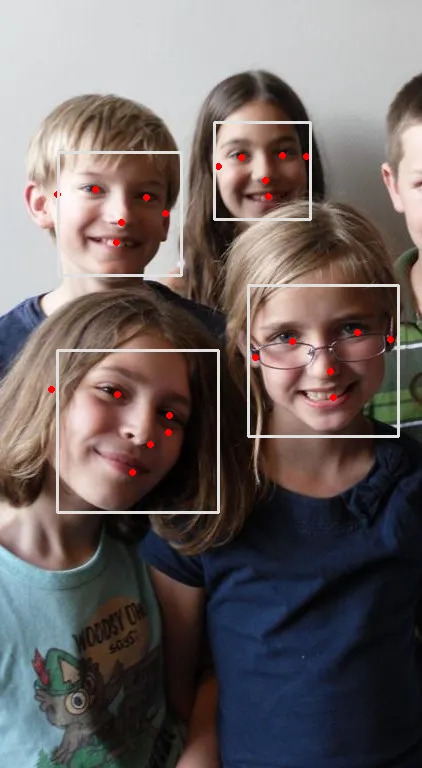
\includegraphics[height=0.7\textheight]{pic/detection_demo.jpg}
            \vfill
        \end{column}
    \end{columns}
\end{frame}

% 1.2
\subsection{技术发展历程}
\begin{frame}{技术发展历程}
\begin{columns}[T]
\begin{column}{0.48\textwidth}
    \textbf{基于手工特征的传统方法}
    \begin{itemize}
        \item 基于知识的方法
        \item 特征不变方法
        \item 模板匹配方法
        \item 基于外观的方法
        \item Viola-Jones 算法 (2001)
        \begin{itemize}
            \item Haar 特征
            \item Adaboost 算法
        \end{itemize}
        \item \dots
    \end{itemize}
\end{column}

\begin{column}{0.48\textwidth}
    \textbf{基于深度学习的方法}
    \begin{itemize}
        \item 多阶段检测架构
        \begin{itemize}
            \item Cascade CNN, MTCNN
        \end{itemize}
        \item 两阶段检测架构
        \begin{itemize}
            \item Face R-CNN, ScaleFace
        \end{itemize}
        \item 单阶段检测架构
        \begin{itemize}
            \item SSD, RetinaNet
        \end{itemize}
    \end{itemize}
\end{column}
\end{columns}
\end{frame}

% 1.3
\subsection{端侧人脸检测}
\begin{frame}{端侧人脸检测}
\begin{block}{端侧设备特点}
\begin{itemize}
    \item 资源受限
    \begin{itemize}
        \item 计算能力有限
        \item 存储容量受限
        \item 功耗要求严格
    \end{itemize}
\end{itemize}
\end{block}

\begin{block}{应用场景}
\begin{itemize}
    \item 手机端
    \begin{itemize}
        \item 自拍美颜
        \item 视频通话人脸跟踪
    \end{itemize}
    \item 嵌入式设备
    \begin{itemize}
        \item 智能安防摄像头
        \item 智能门禁系统
    \end{itemize}
\end{itemize}
\end{block}
\end{frame}
% 第二章
\section{轻量化卷积网络}

% 2.1
% \subsection{概述}
\begin{frame}{轻量化卷积网络概述}
    \begin{itemize}
        \item 负责提取图像特征
        \item 直接影响模型效率和准确性
        \item 主流轻量化卷积网络:
        \begin{itemize}
            \item SqueezeNet (2016.02)
            \item MobileNets (2017.04)
            \item ShuffleNet (2017.07)
            \item 其他:Xception、EfficientNet、GhostNet 等
        \end{itemize}
        \item 特别说明:本次介绍仅涉及各网络的初始版本
    \end{itemize}
\end{frame}

% 2.2 SqueezeNet
\subsection{SqueezeNet}
\begin{frame}{SqueezeNet 架构}
    \begin{block}{主要特点}
        \begin{itemize}
            \item 2016 年 2 月由伯克利和斯坦福研究人员提出,是较早提出的一个轻量化神经网络
            \item 在保持和 AlexNet 相同准确率的情况下,将模型参数减少到原来的 50 倍
            \item 压缩后仅 0.47MB
        \end{itemize}
    \end{block}
    \begin{block}{三个设计策略}
        \begin{enumerate}
            \item 用 1$\times$1 卷积替代 3$\times$3 卷积
            \item 减少 3$\times$3 卷积的输入通道数
            \item 延迟下采样,保持较大特征图尺寸
        \end{enumerate}
    \end{block}
\end{frame}

\begin{frame}{Fire Module}
    \begin{itemize}
        \item 核心组成部分:
        \begin{itemize}
            \item squeeze 层: 使用 1$\times$1 卷积压缩特征图通道数
            \item expand 层: 使用 1$\times$1 和 3$\times$3 卷积提升通道数并拼接结果
        \end{itemize}
    \end{itemize}
    \begin{figure}
        \centering
        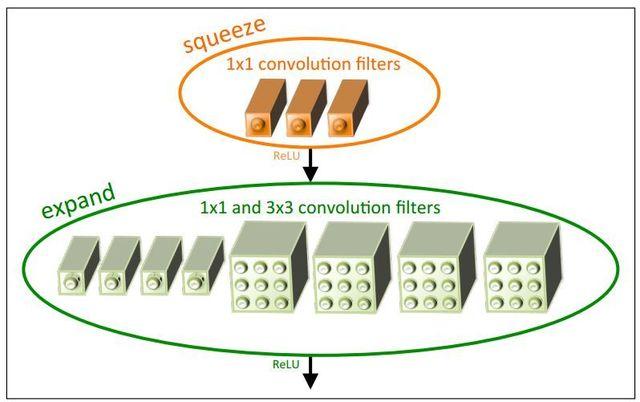
\includegraphics[width=0.7\linewidth]{pic/fire_module.jpg}
        \caption{Fire Module 结构}
    \end{figure}
\end{frame}

\begin{frame}{SqueezeNet 性能对比}
    \begin{figure}
        \centering
        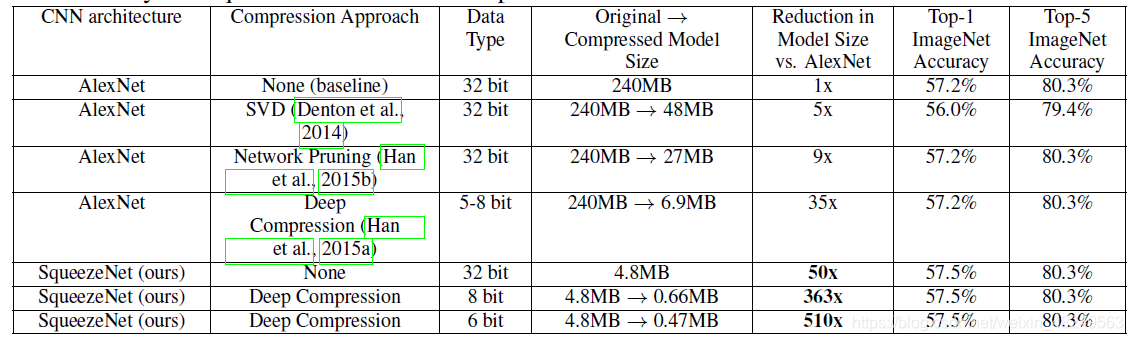
\includegraphics[width=0.8\linewidth]{pic/squeezenet_vs_alexnet.png}
        \caption{SqueezeNet 与 AlexNet 在 ImageNet 上的对比}
    \end{figure}
    
    \begin{itemize}
        \item 在 ImageNet 数据集上的 TOP-1 和 TOP-5 的准确率都与 AlexNet 相似
        \item SqueezeNet 模型参数量仅为 AlexNet 的 1/50,压缩后模型文件仅 0.47MB
    \end{itemize}
\end{frame}

% 2.3 MobileNet
\subsection{MobileNet}
\begin{frame}{MobileNet 架构}

    \begin{itemize}
        \item 2017 年 4 月由 Google 团队提出
        \item 基于流线型架构,提出深度可分离卷积构建轻量级深层神经网络,在减少模型参数两的同时保持良好的特征提取能力。
        \item 深度可分离卷积的两个步骤:
        \begin{itemize}
            \item 深度卷积 (Depthwise Conv):每个通道独立卷积,实现空间信息的提取
            \item 逐点卷积 (Pointwise Conv):1$\times$1 卷积融合通道信息,确保每个输出特征图包含所有输入特征图的信息
        \end{itemize}
    \end{itemize}

    \begin{figure}
        \centering
        \begin{subfigure}[b]{0.32\textwidth}
            \centering
            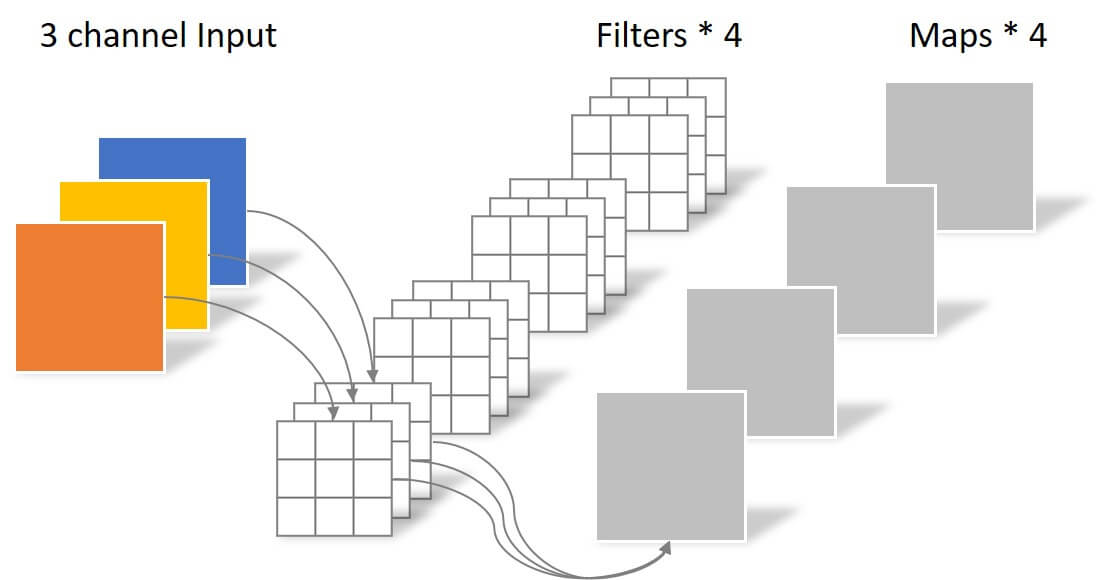
\includegraphics[width=\linewidth]{pic/std_cov.jpg}
            \caption{标准卷积}
        \end{subfigure}
        \begin{subfigure}[b]{0.32\textwidth}
            \centering
            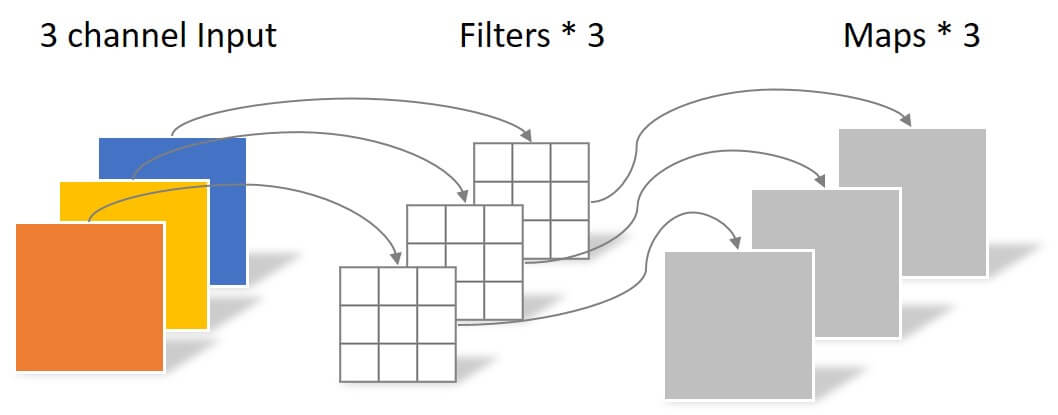
\includegraphics[width=\linewidth]{pic/dpth_cov.jpg}
            \caption{深度卷积}
        \end{subfigure}
        \begin{subfigure}[b]{0.32\textwidth}
            \centering
            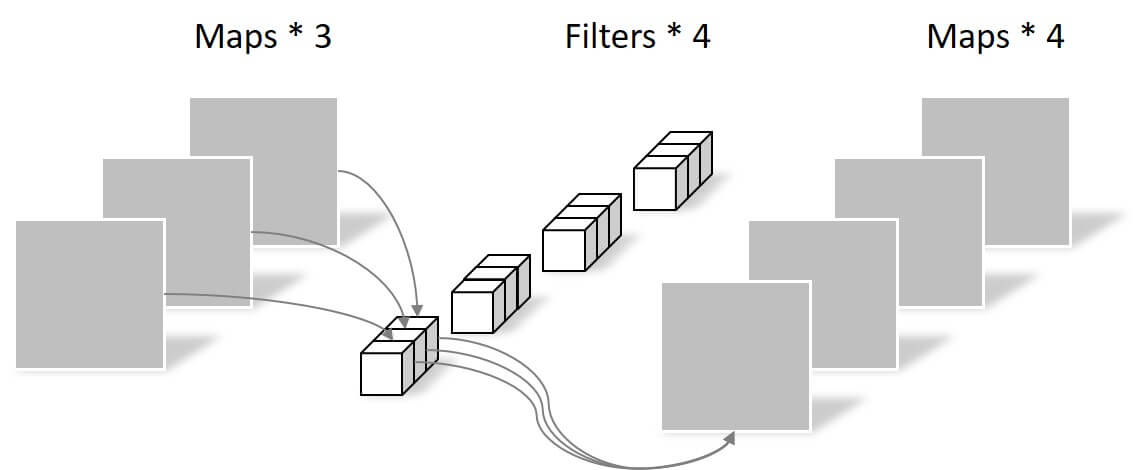
\includegraphics[width=\linewidth]{pic/sep_cov.jpg}
            \caption{逐点卷积}
        \end{subfigure}
    \end{figure}
\end{frame}

\begin{frame}{深度可分离卷积参数量分析}
    \begin{block}{参数量}
        \begin{equation*}
            P_{std} = K \times K \times C \times N = K^2 \times C \times N
        \end{equation*}
        \begin{equation*}
            P_{ds} = (K \times K \times N) + (1 \times 1 \times C \times N) = (K^2 + C) \times N
        \end{equation*}
    \end{block}
    
    \begin{block}{压缩比}
        \begin{equation*}
            \frac{P_{ds}}{P_{std}} = \frac{(K^2 + C) \times N}{K^2 \times C \times N} = \frac{1}{C} + \frac{1}{K^2}
        \end{equation*}
    \end{block}
    当$K=3$时,压缩比约为 9 倍
\end{frame}

\begin{frame}{MobileNet 性能对比}
    \begin{figure}
        \centering
        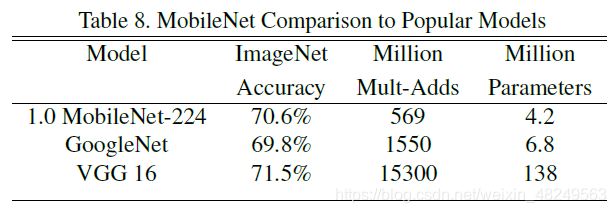
\includegraphics[width=0.8\linewidth]{pic/mobilenet_comp.png}
        \caption{MobileNet 与其他模型在 ImageNet 上的性能对比}
    \end{figure}
    
    \begin{itemize}
        \item 精度略高于 GoogLeNet,但计算量仅为其 1/3
        \item 相比 VGG-16 精度降低 0.9\%,但参数量和计算量大幅降低
    \end{itemize}
\end{frame}

% 2.4 ShuffleNet
\subsection{ShuffleNet}
\begin{frame}{ShuffleNet}

    \begin{itemize}
        \item 2017 年 7 月由 Face++团队(旷世科技)提出
        \item MobileNet 中 $1 \times 1$ 卷积耗费了 94.8\% 的计算时间
        \item 提出逐点分组卷积 (Pointwise Group Convolution) 减少计算时间
        \item 通过通道重排 (Channel Shuffle) 解决分组卷积信息交互问题
        \item 在相同参数量规模下,ShuffleNet 在 ImageNet 数据集上的 TOP-1 准确率高于 MobileNet
    \end{itemize}

    \begin{figure}
        \centering
        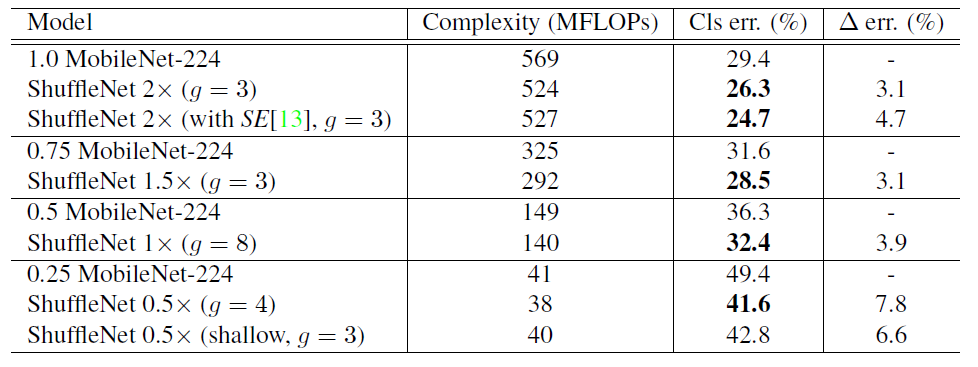
\includegraphics[width=0.6\linewidth]{pic/shufflenet_comp.png}
        \caption{ShuffleNet 与其他模型在 ImageNet 上的性能对比}
    \end{figure}
\end{frame}

% 第三章
\section{轻量级人脸检测模型}

% 3.1 概述
\begin{frame}{轻量级人脸检测模型概述}
    \begin{itemize}
        \item 本研究选择三个代表性模型:
        \begin{itemize}
            \item RetinaFace (2019)
            \item BlazeFace (2019)
            \item YOLO5Face (2021)
        \end{itemize}
        \item 选择标准:
        \begin{itemize}
            \item 模型轻量化,实时性能好
            \item 在如今端侧轻量化模型实践中应用广泛
            \item 在 WiderFace 数据集取得较高排名
        \end{itemize}
    \end{itemize}
\end{frame}

% 3.2 RetinaFace
\subsection{RetinaFace}
\begin{frame}{RetinaFace}
    \begin{block}{主要特点}
        \begin{itemize}
            \item 2019 年由 Insight Face 团队提出,曾长期保持 SOTA 水平
            \item 采用多任务学习框架,结合监督学习和自监督学习
            \item 支持不同 backbone 选择,可平衡精度和速度
            \item 支持人脸检测、关键点定位和密集人脸对应关系预测
        \end{itemize}
    \end{block}

    \begin{block}{实验选用版本}
        \begin{itemize}
            \item RetinaFace-MobileNet0.25
            \item RetinaFace-MobileNetV2
            \item 可直接对原始图片进行推理,无需预处理缩放
        \end{itemize}
    \end{block}
\end{frame}

% 3.3 BlazeFace
\subsection{BlazeFace}
\begin{frame}{BlazeFace 特点}
    \begin{itemize}
        \item Google 专为移动 GPU 优化设计
        \item Google ML Kit 和 MediaPipe 默认人脸检测模型
        \item 在 iPhone XS 上推理时间仅需 0.6ms
        \item 基于 MobileNetV1/V2 定制特征提取网络
        \item 提出适合 GPU 运算的新型 anchor 方案
        \item 改进 NMS 策略,提高视频检测稳定性
    \end{itemize}
\end{frame}
\begin{frame}{BlazeFace 实验选用版本}
    \begin{itemize}
        \item BlazeFace-128 为前置摄像头设计,接收 128$\times$128 的输入
        \item BlazeFace-320 和 BlazeFace-640 分别接受 320$\times$320 和 640$\times$640 的输入
        \item 采用 padding 方式等比例缩放
        \item 比 MobileNetV2-SSD 快近 4 倍
        \item 支持人脸关键点预测和旋转角度估计
    \end{itemize}
\end{frame}

% 3.4 YOLO5Face
\subsection{YOLO5Face}
\begin{frame}{YOLO5Face}
    \begin{block}{主要特点}
        \begin{itemize}
            \item 将人脸检测视为通用目标检测任务
            \item 基于 YOLOv5 增加关键点回归功能并改进网络结构
            \item 在 WiderFace 数据集上性能优异,超过许多专门的人脸检测模型
        \end{itemize}
    \end{block}
    
    \begin{block}{实验选用版本}
        \begin{itemize}
            \item YOLO5Face 基于 ShuffleNetv2 设计轻量级模型,优化网络架构大幅缩小模型体积
            \item 本次实验使用 YOLOv5n 和 YOLOv5n-0.5 两个版本
            \item 输入尺寸:640$\times$640,采用 padding 方式等比例缩放
            \item 非常适合在嵌入式设备和移动设备上部署
        \end{itemize}
    \end{block}
\end{frame}

% 第四章
\section{模型对比试验}

% 4.1 实验设计
\subsection{实验设计}
\begin{frame}{实验环境}

    \begin{figure}[h]
        \centering
        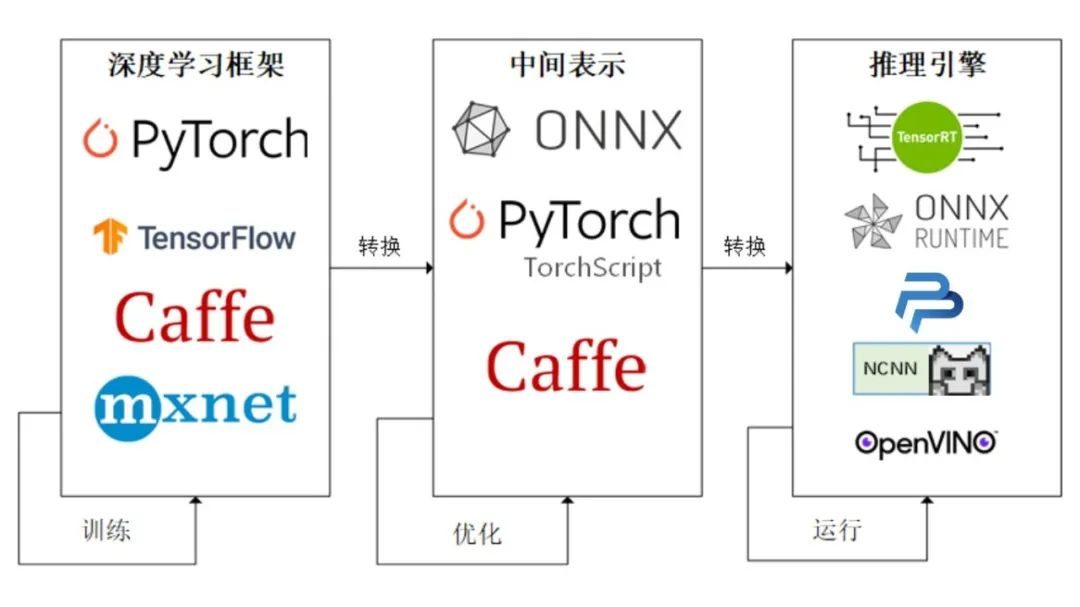
\includegraphics[width=0.6\textwidth]{pic/pipeline.jpg}
        \caption{ONNX模型转换流程}
    \end{figure}

    \begin{itemize}
        \item 统一导出为ONNX格式
        \item 使用ONNX Runtime作为推理引擎
        \item 硬件: i5-10400 CPU (0.5TFLOPS)
    \end{itemize}
\end{frame}

\begin{frame}{评估指标}
    \begin{itemize}
        \item 检测精度: 使用标准评估代码计算各模型在 WIDER FACE 数据集上的精度,同时在自建数据集 light\_face 上计算 mAP
        \item 计算效率: 在 ONNX Runtime 上测试推理时延
        \item 模型大小: 对比导出为 ONNX 格式后各模型的大小
    \end{itemize}
\end{frame}

% 4.2 数据集
\subsection{数据集}
\begin{frame}{实验数据集}
    \begin{block}{WIDER FACE验证集}
        \begin{itemize}
            \item 人脸检测领域标准基准数据集
            \item 具有广泛代表性和权威性
            \item 提供了标准的评估代码
        \end{itemize}
    \end{block}

    \begin{block}{自建单人人脸数据集 light\_face}
        \begin{itemize}
            \item 通过笔记本和手机前置摄像头采集,考虑姿态角度和光照变化
            \item 约1000张图像样本
            \item 贴近端侧实际应用场景
            \item 使用腾讯云API进行标注
        \end{itemize}
    \end{block}
\end{frame}

% 4.3 实验结果
\subsection{实验结果}
\begin{frame}{模型性能对比}
    \begin{table}
        \centering
        \caption{各模型性能指标对比}
        \scalebox{0.8}{
            \begin{tabular}{l|c|c|c|c|c|c}
                \hline
                Model & Size(MB) & FPS & Easy & Medium & Hard & light\_face \\
                \hline
                retinaface\_mv1 & 1.66 & 8.68 & 0.91 & 0.88 & 0.73 & \underline{0.99} \\
                retinaface\_mv2 & 11.93 & 4.15 & 0.94 & \underline{0.92} & \underline{0.82} & 0.99 \\
                yolov5n\_0.5\_face & 5.65 & 22.23 & 0.91 & 0.88 & 0.75 & 0.99 \\
                yolov5n\_face & 10.51 & 12.90 & \underline{0.94} & 0.92 & 0.81 & 0.99 \\
                blazeface\_128 & \underline{0.44} & \underline{70.79} & 0.18 & 0.10 & 0.04 & 0.67 \\
                blazeface\_320 & 0.68 & 46.46 & 0.60 & 0.46 & 0.20 & 0.93 \\
                blazeface\_640 & 0.68 & 16.26 & 0.80 & 0.64 & 0.35 & 0.98 \\
                \hline
            \end{tabular}
        }
    \end{table}

    \begin{itemize}
        \item RetinaFace和YOLOv5系列精度高但模型较大
        \item BlazeFace系列速度快且轻量,但精度有所牺牲
        \item yolov5n\_0.5\_face 在模型大小、计算效率和精度上表现均衡
    \end{itemize}
\end{frame}

\begin{frame}{模型性能数据分析 - 模型大小与速度}
    \begin{figure}
        \centering
        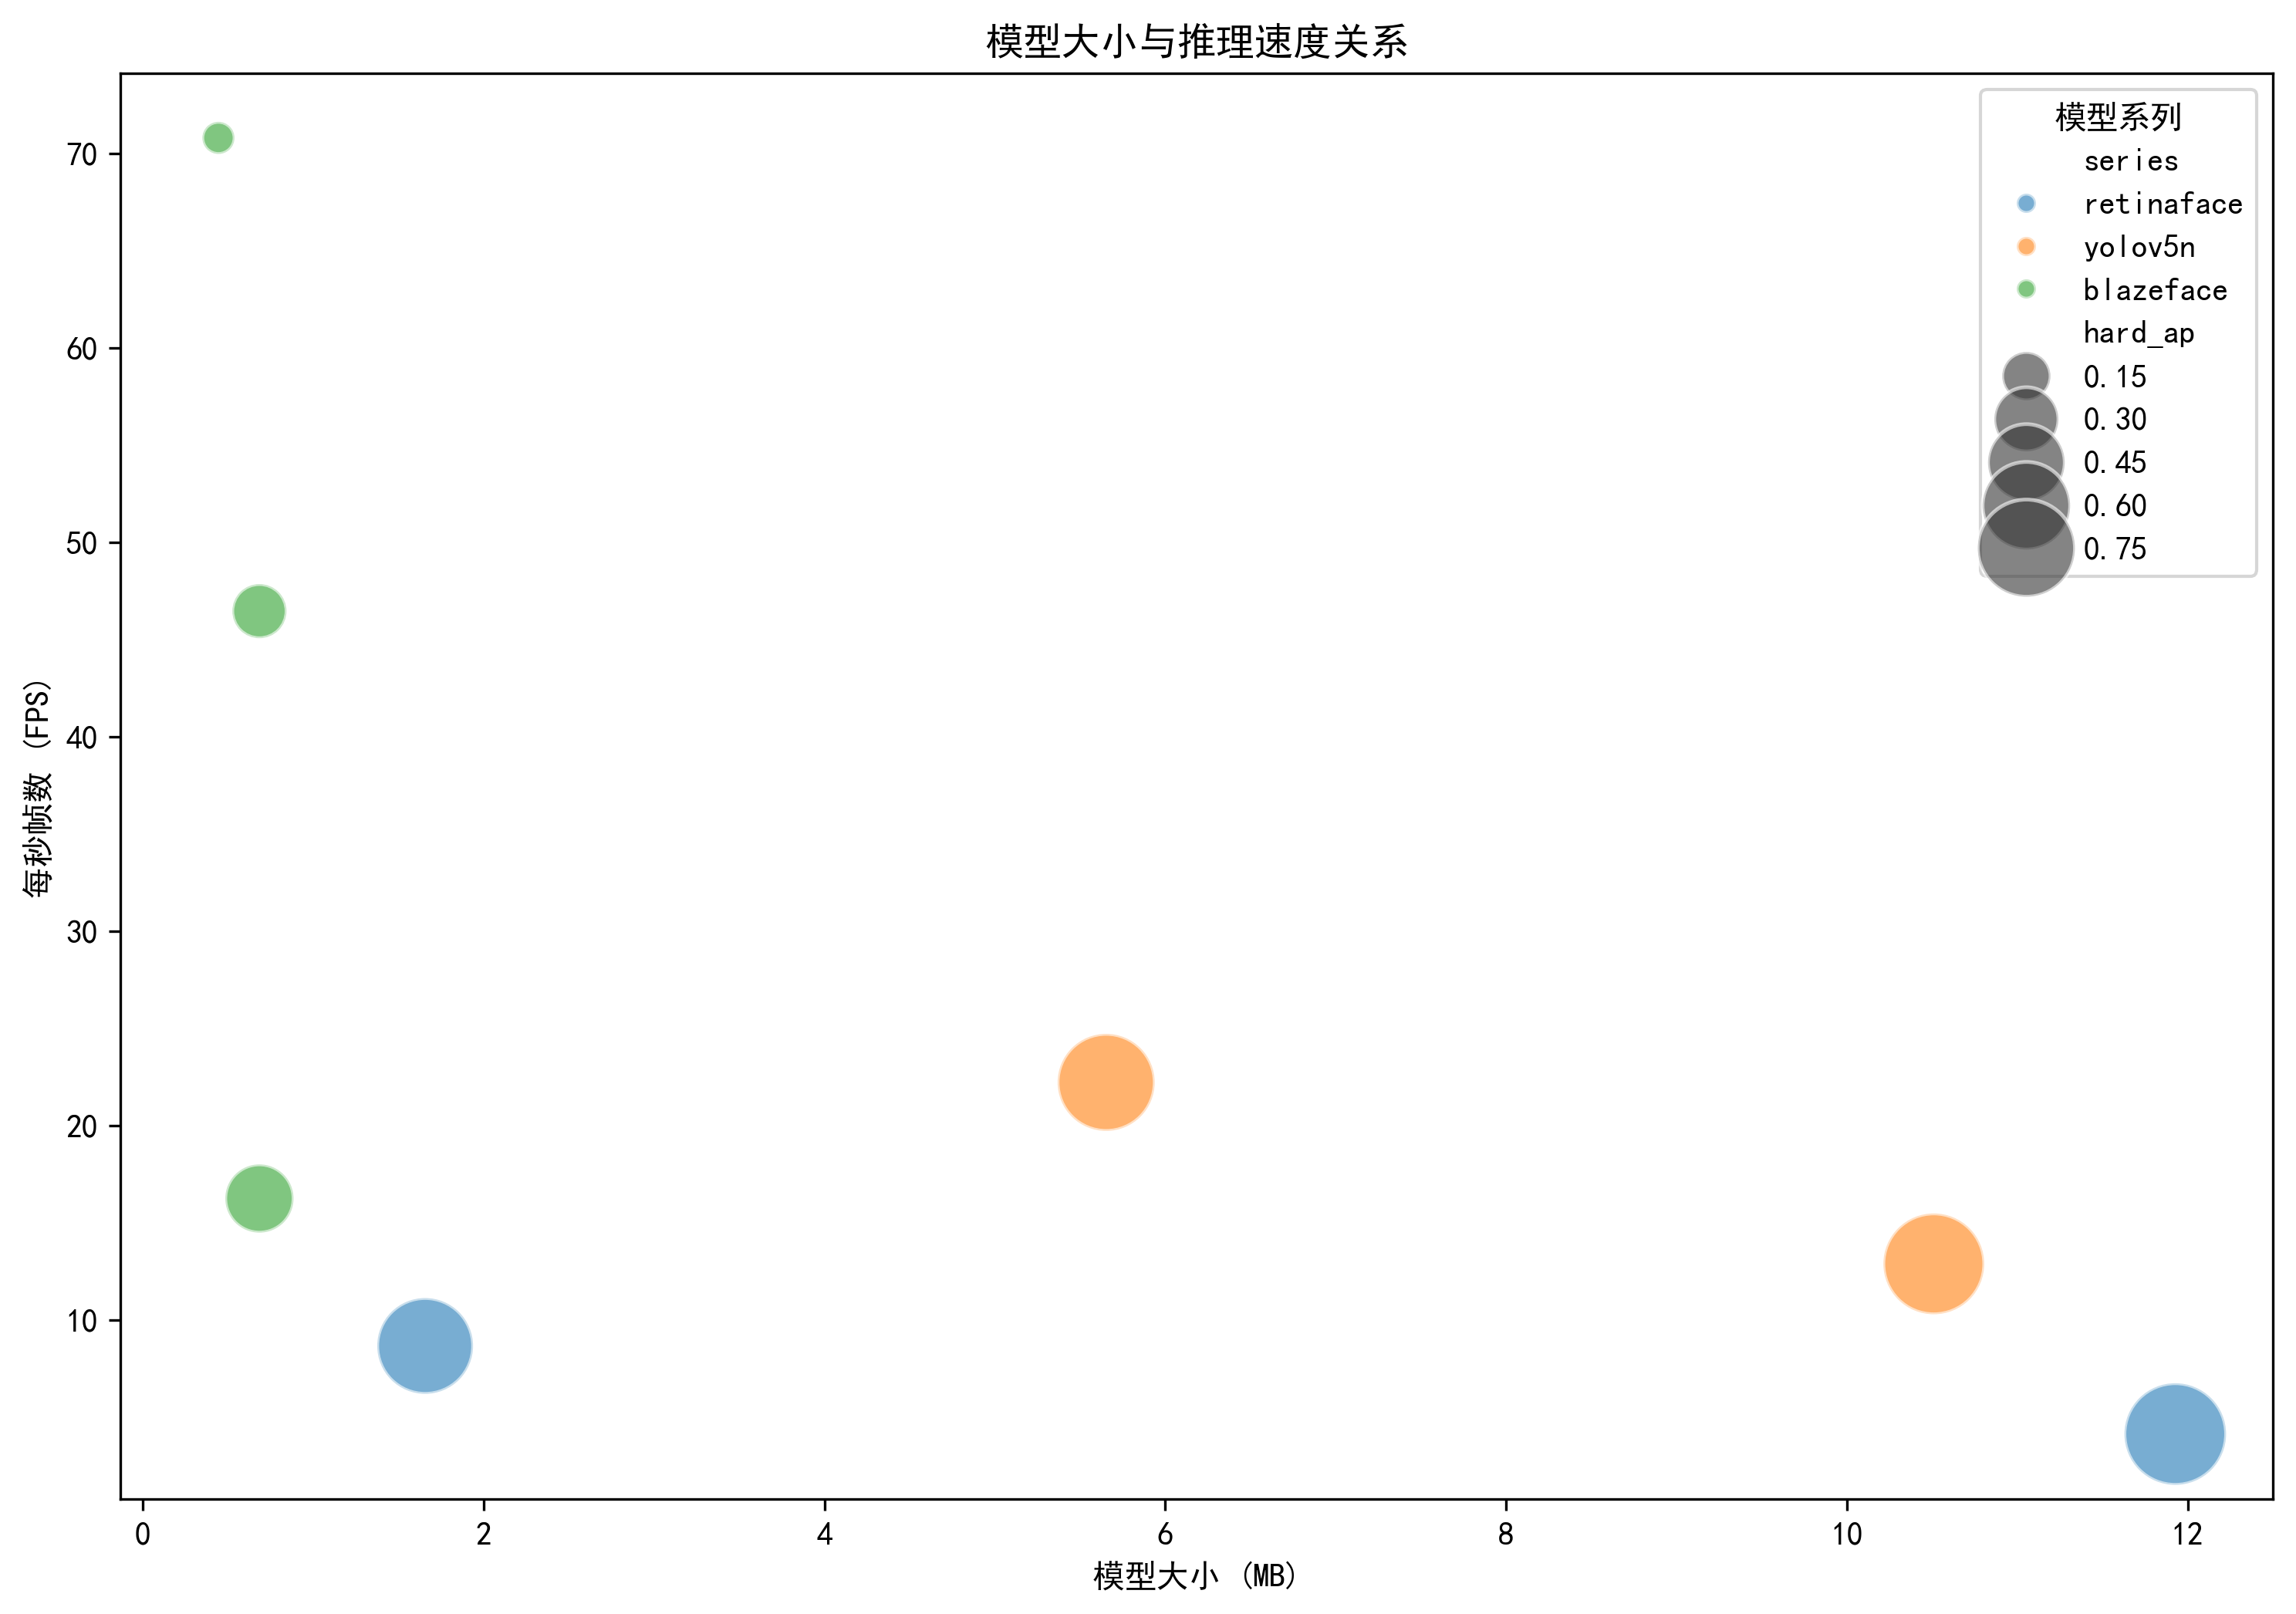
\includegraphics[width=0.7\textwidth]{pic/size_fps.png}
        \caption{模型大小与推理速度对比}
    \end{figure}
\end{frame}
\begin{frame}{模型性能数据分析 - 检测精度}
    \begin{columns}
        \begin{column}{0.5\textwidth}
            \begin{figure}
                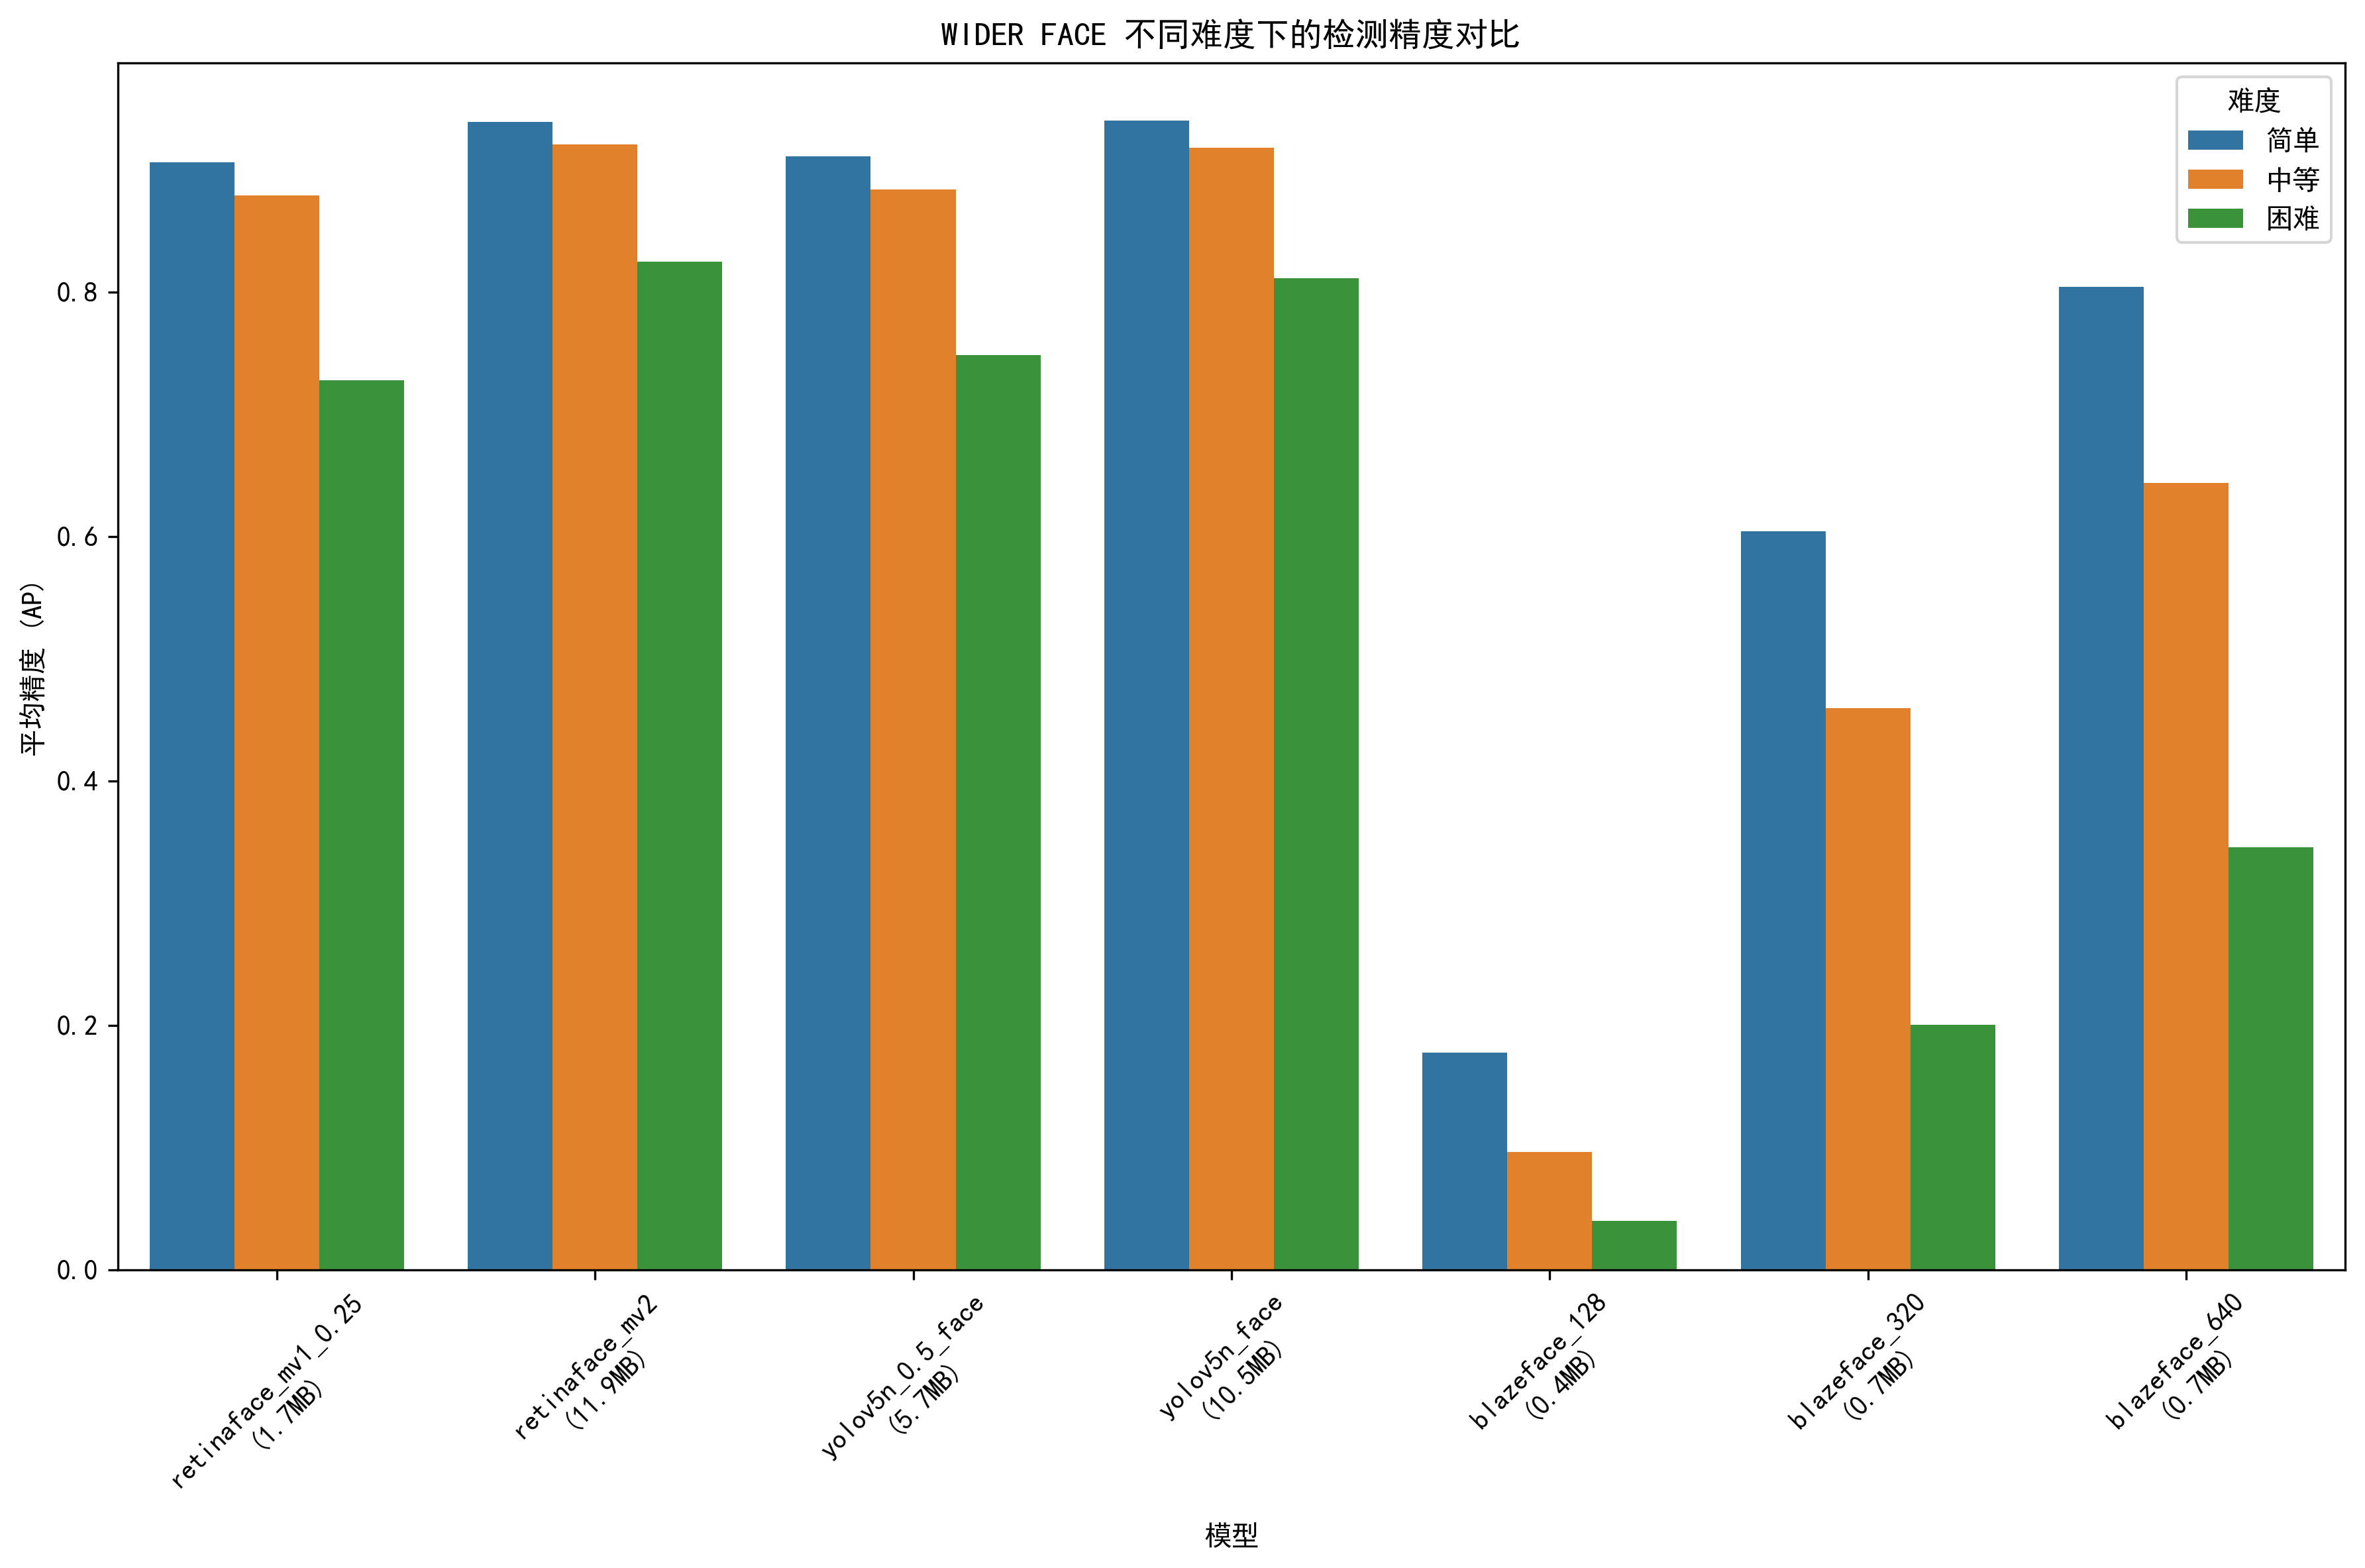
\includegraphics[width=\textwidth]{pic/ap_comparison.png}
                \caption{不同难度级别下的检测精度对比}
            \end{figure}
        \end{column}
        \begin{column}{0.5\textwidth}
            \begin{figure}
                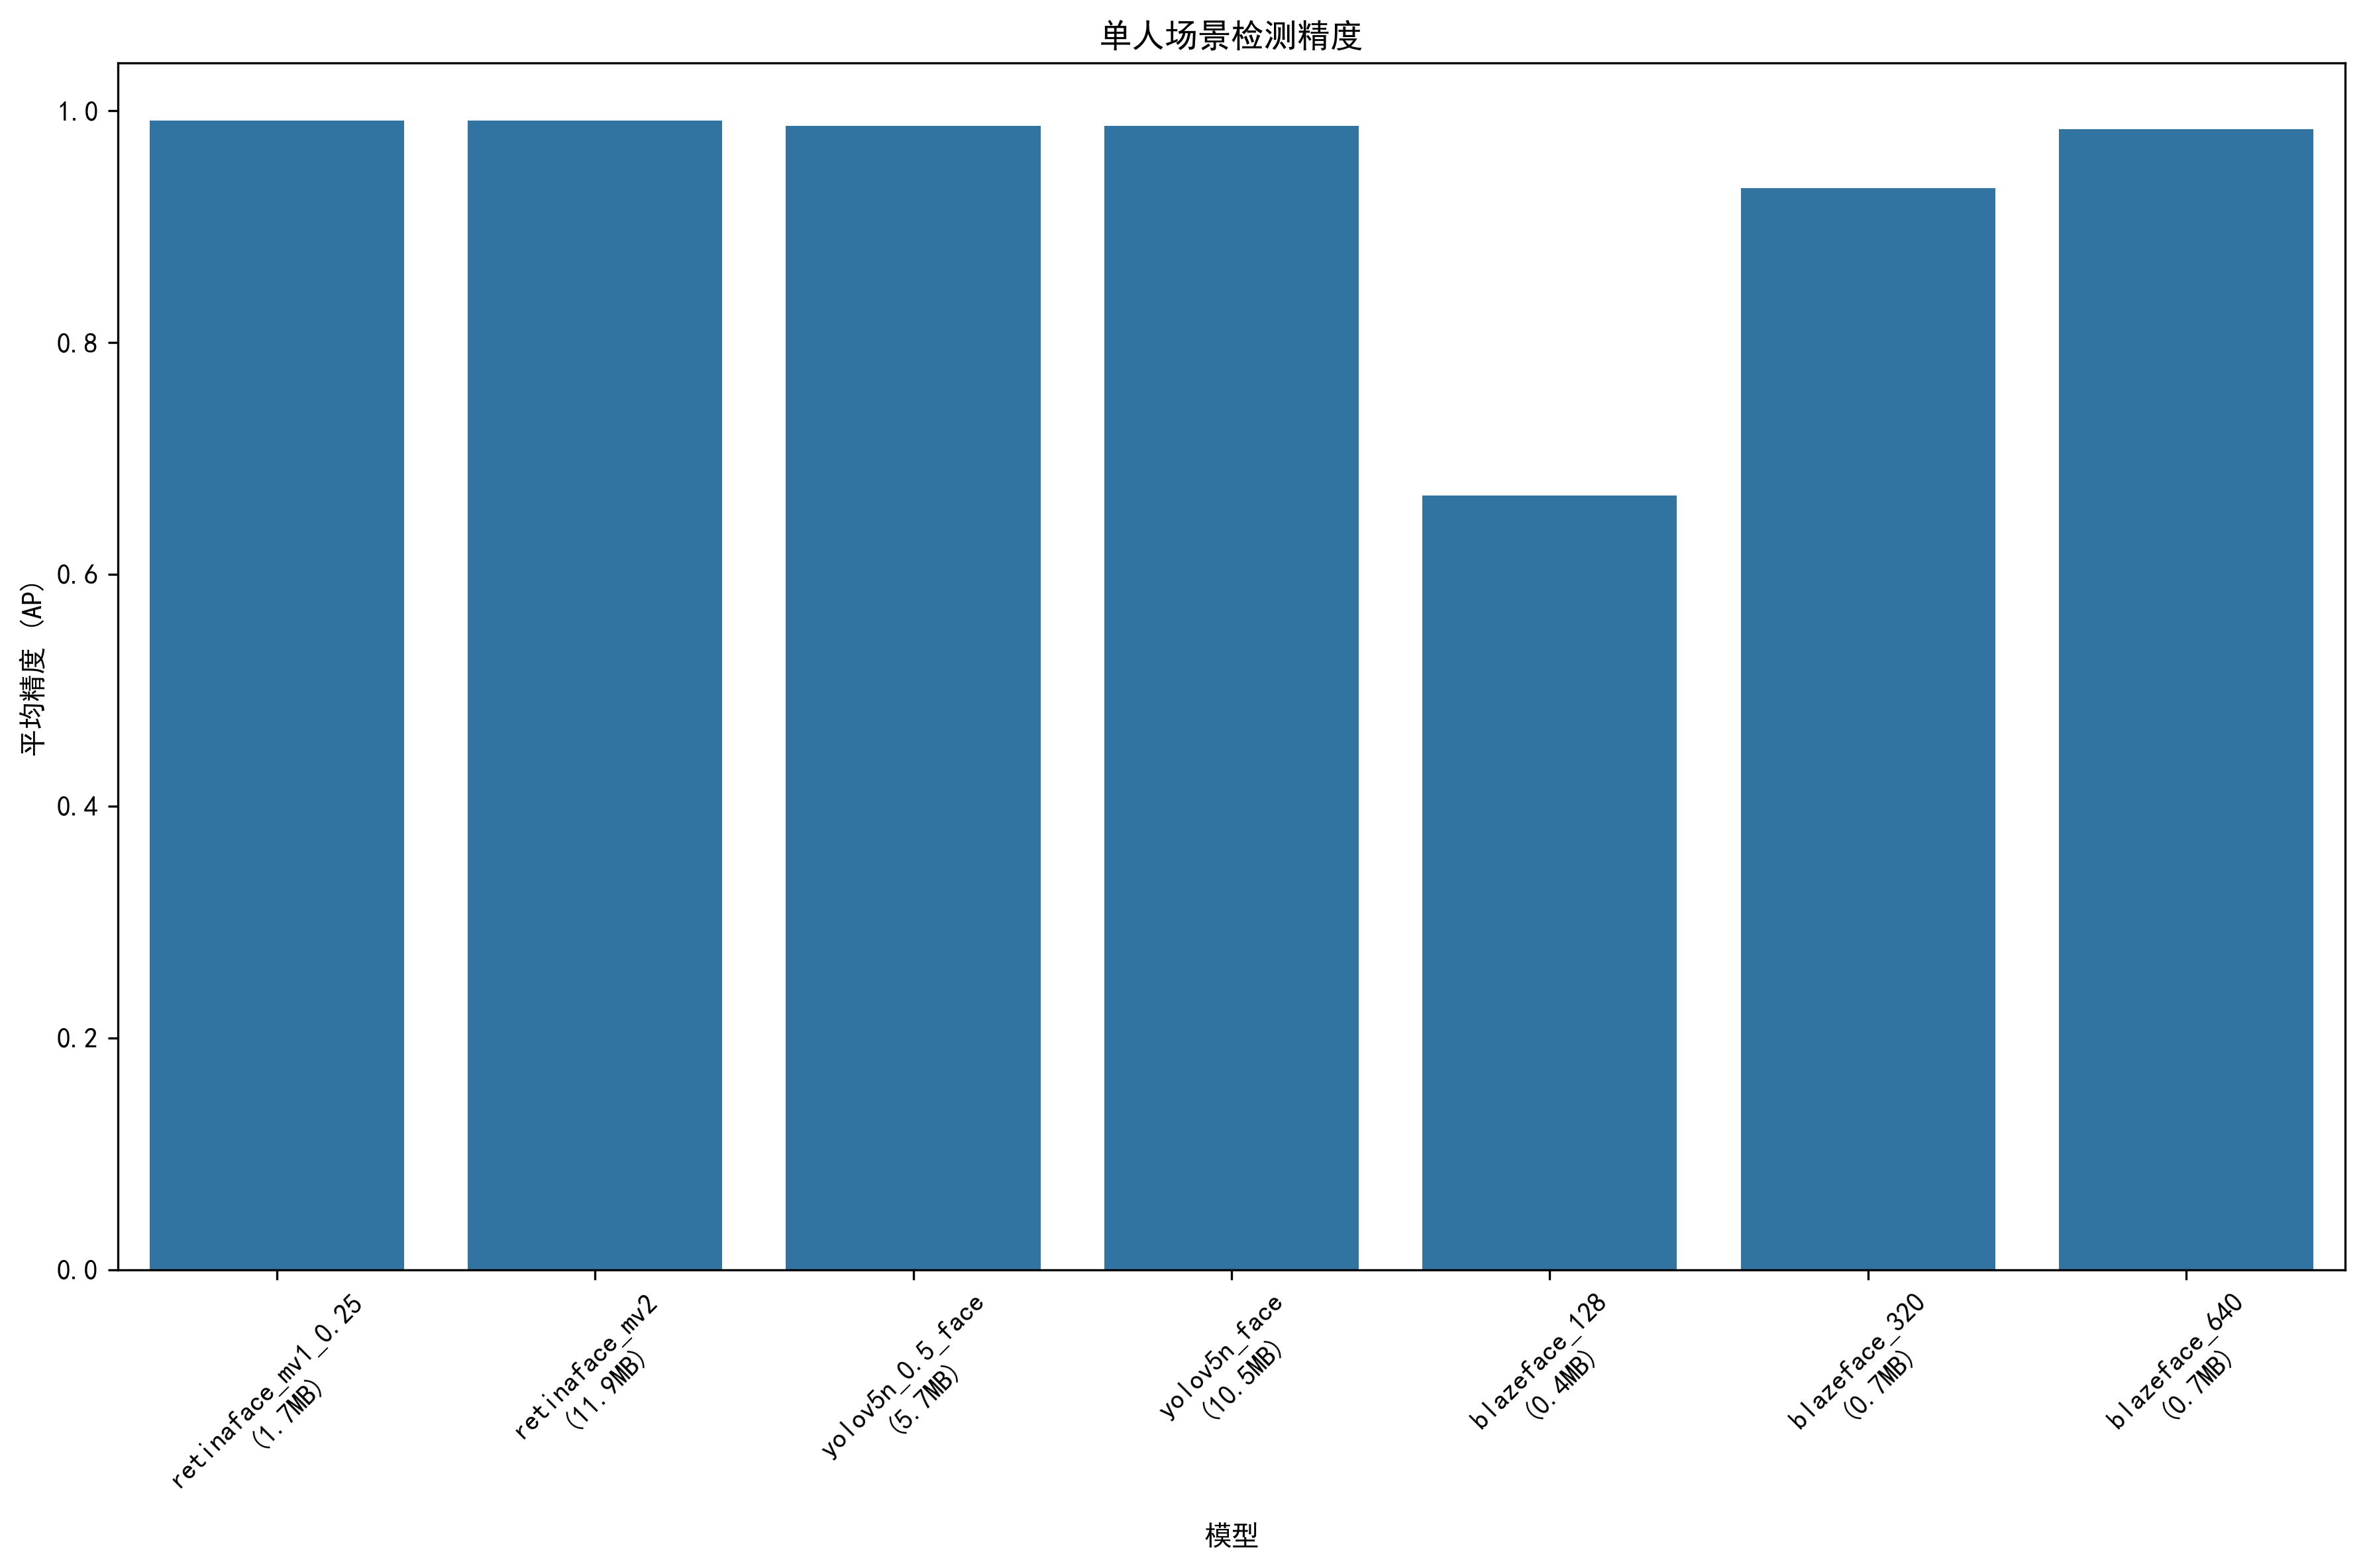
\includegraphics[width=\textwidth]{pic/one_face_ap.png}
                \caption{单人人脸场景下的检测精度对比}
            \end{figure}
        \end{column}
    \end{columns}
\end{frame}


\begin{frame}{应用场景建议}
    \begin{block}{高精度场景}
        \begin{itemize}
            \footnotesize
            \item 推荐: YOLOv5n\_face 或 RetinaFace\_mv2
            \item 特点: 各难度级别AP值均高(>0.81)
            \item 代价: 模型较大(10-12MB),速度较慢(4-13FPS)
            \item 适用: 安防监控,门禁考勤等
        \end{itemize}
    \end{block}

    \begin{block}{移动端前置摄像头}
        \begin{itemize}
            \footnotesize
            \item 推荐: BlazeFace\_320
            \item 特点: 体积小(0.68MB),速度快(46FPS),单人人脸识别场景AP达0.93
            \item 代价: 非单人场景下精度较低(0.6-0.8)
            \item 适用: 移动端实时检测场景,相机应用、视频会议、AR 试妆等
        \end{itemize}
    \end{block}
\end{frame}


\begin{frame}{应用场景建议}
    \begin{block}{轻量级场景}
        \begin{itemize}
            \footnotesize
            \item 推荐: BlazeFace\_128
            \item 特点: 最小体积(0.44MB),最快速度(70+FPS),在 light\_face 数据集上精度尚可(0.67)
            \item 代价: 精度较低(0.18-0.6)
            \item 适用: 资源受限的 IoT 设备,例如智能门锁、手表、玩具等
        \end{itemize}
    \end{block}
    \begin{block}{平衡场景}
        \begin{itemize}
            \footnotesize
            \item 推荐: YOLOv5n\_0.5\_face
            \item 特点: 中等体积(5MB),较快速度(25FPS),各难度级别AP值均衡(0.7-0.8)
            \item 代价: 在各方面都不是最优
            \item 适用: 需要在资源和性能间取得平衡的场景,如移动端后置摄像头应用
        \end{itemize}
    \end{block}
\end{frame}

% 致谢页
%\section{致谢}
\begin{frame}
    \begin{center}
        {\Huge\calligra 感谢各位的聆听}
    \end{center}
\end{frame}

\end{document}